\documentclass[twocolumn]{svjour3}
\smartqed
\usepackage{graphicx}
\usepackage{microtype}
\usepackage{amsmath}
\usepackage{amssymb}
\usepackage{booktabs}
\usepackage{url}
\newcommand{\MaePIDS}{55.51}
\newcommand{\MaeSdPIDS}{1.80}
\newcommand{\NMaePIDS}{3}
\newcommand{\PeakPIDS}{2.71}
\newcommand{\PeakSdPIDS}{0.03}
\newcommand{\NPeakPIDS}{3}
\newcommand{\ChatPIDS}{0.005}
\newcommand{\ChatSdPIDS}{0.00}
\newcommand{\NChatPIDS}{3}
\newcommand{\StatPIDS}{26.08}
\newcommand{\StatSdPIDS}{0.11}
\newcommand{\NStatPIDS}{3}
\newcommand{\LowPIDS}{49.83}
\newcommand{\LowSdPIDS}{0.18}
\newcommand{\NLowPIDS}{3}
\newcommand{\LowRecPIDS}{--}
\newcommand{\LowRecSdPIDS}{--}
\newcommand{\NLowRecPIDS}{0}
\newcommand{\LowBurstPIDS}{32.51}
\newcommand{\LowBurstSdPIDS}{0.12}
\newcommand{\NLowBurstPIDS}{3}
\newcommand{\SyncPIDS}{8.25}
\newcommand{\SyncSdPIDS}{0.09}
\newcommand{\NSyncPIDS}{3}
\newcommand{\MaePITS}{9.55}
\newcommand{\MaeSdPITS}{0.15}
\newcommand{\NMaePITS}{6}
\newcommand{\PeakPITS}{1.88}
\newcommand{\PeakSdPITS}{0.09}
\newcommand{\NPeakPITS}{6}
\newcommand{\ChatPITS}{0.043}
\newcommand{\ChatSdPITS}{0.00}
\newcommand{\NChatPITS}{6}
\newcommand{\StatPITS}{1.32}
\newcommand{\StatSdPITS}{0.08}
\newcommand{\NStatPITS}{3}
\newcommand{\LowPITS}{28.78}
\newcommand{\LowSdPITS}{0.17}
\newcommand{\NLowPITS}{6}
\newcommand{\LowRecPITS}{1.83}
\newcommand{\LowRecSdPITS}{0.41}
\newcommand{\NLowRecPITS}{6}
\newcommand{\LowBurstPITS}{10.43}
\newcommand{\LowBurstSdPITS}{0.53}
\newcommand{\NLowBurstPITS}{6}
\newcommand{\SyncPITS}{8.52}
\newcommand{\SyncSdPITS}{0.01}
\newcommand{\NSyncPITS}{6}
\newcommand{\MaePIFFS}{1.25}
\newcommand{\MaeSdPIFFS}{0.17}
\newcommand{\NMaePIFFS}{15}
\newcommand{\PeakPIFFS}{1.36}
\newcommand{\PeakSdPIFFS}{0.05}
\newcommand{\NPeakPIFFS}{15}
\newcommand{\ChatPIFFS}{0.055}
\newcommand{\ChatSdPIFFS}{0.01}
\newcommand{\NChatPIFFS}{15}
\newcommand{\StatPIFFS}{1.38}
\newcommand{\StatSdPIFFS}{0.08}
\newcommand{\NStatPIFFS}{3}
\newcommand{\LowPIFFS}{31.48}
\newcommand{\LowSdPIFFS}{0.30}
\newcommand{\NLowPIFFS}{6}
\newcommand{\LowRecPIFFS}{24.08}
\newcommand{\LowRecSdPIFFS}{1.16}
\newcommand{\NLowRecPIFFS}{6}
\newcommand{\LowBurstPIFFS}{16.55}
\newcommand{\LowBurstSdPIFFS}{0.78}
\newcommand{\NLowBurstPIFFS}{6}
\newcommand{\SyncPIFFS}{8.67}
\newcommand{\SyncSdPIFFS}{0.00}
\newcommand{\NSyncPIFFS}{15}
\newcommand{\MaeFFOS}{1.82}
\newcommand{\MaeSdFFOS}{0.30}
\newcommand{\NMaeFFOS}{15}
\newcommand{\PeakFFOS}{1.34}
\newcommand{\PeakSdFFOS}{0.07}
\newcommand{\NPeakFFOS}{15}
\newcommand{\ChatFFOS}{0.032}
\newcommand{\ChatSdFFOS}{0.01}
\newcommand{\NChatFFOS}{15}
\newcommand{\StatFFOS}{1.34}
\newcommand{\StatSdFFOS}{0.25}
\newcommand{\NStatFFOS}{3}
\newcommand{\LowFFOS}{28.18}
\newcommand{\LowSdFFOS}{0.17}
\newcommand{\NLowFFOS}{6}
\newcommand{\LowRecFFOS}{2.92}
\newcommand{\LowRecSdFFOS}{0.74}
\newcommand{\NLowRecFFOS}{6}
\newcommand{\LowBurstFFOS}{8.85}
\newcommand{\LowBurstSdFFOS}{0.51}
\newcommand{\NLowBurstFFOS}{6}
\newcommand{\SyncFFOS}{8.61}
\newcommand{\SyncSdFFOS}{0.01}
\newcommand{\NSyncFFOS}{15}
\newcommand{\MaeMPCPS}{1.69}
\newcommand{\MaeSdMPCPS}{0.28}
\newcommand{\NMaeMPCPS}{15}
\newcommand{\PeakMPCPS}{1.36}
\newcommand{\PeakSdMPCPS}{0.04}
\newcommand{\NPeakMPCPS}{15}
\newcommand{\ChatMPCPS}{0.026}
\newcommand{\ChatSdMPCPS}{0.01}
\newcommand{\NChatMPCPS}{15}
\newcommand{\StatMPCPS}{1.22}
\newcommand{\StatSdMPCPS}{0.11}
\newcommand{\NStatMPCPS}{3}
\newcommand{\LowMPCPS}{28.01}
\newcommand{\LowSdMPCPS}{0.60}
\newcommand{\NLowMPCPS}{6}
\newcommand{\LowRecMPCPS}{3.00}
\newcommand{\LowRecSdMPCPS}{0.32}
\newcommand{\NLowRecMPCPS}{6}
\newcommand{\LowBurstMPCPS}{8.98}
\newcommand{\LowBurstSdMPCPS}{0.22}
\newcommand{\NLowBurstMPCPS}{6}
\newcommand{\SyncMPCPS}{8.61}
\newcommand{\SyncSdMPCPS}{0.00}
\newcommand{\NSyncMPCPS}{15}
\newcommand{\MaeMPCMS}{2.81}
\newcommand{\MaeSdMPCMS}{0.45}
\newcommand{\NMaeMPCMS}{10}
\newcommand{\PeakMPCMS}{1.50}
\newcommand{\PeakSdMPCMS}{0.08}
\newcommand{\NPeakMPCMS}{10}
\newcommand{\ChatMPCMS}{0.024}
\newcommand{\ChatSdMPCMS}{0.01}
\newcommand{\NChatMPCMS}{10}
\newcommand{\StatMPCMS}{1.31}
\newcommand{\StatSdMPCMS}{0.10}
\newcommand{\NStatMPCMS}{3}
\newcommand{\LowMPCMS}{28.22}
\newcommand{\LowSdMPCMS}{0.11}
\newcommand{\NLowMPCMS}{6}
\newcommand{\LowRecMPCMS}{2.33}
\newcommand{\LowRecSdMPCMS}{0.82}
\newcommand{\NLowRecMPCMS}{6}
\newcommand{\LowBurstMPCMS}{8.92}
\newcommand{\LowBurstSdMPCMS}{0.28}
\newcommand{\NLowBurstMPCMS}{6}
\newcommand{\SyncMPCMS}{8.60}
\newcommand{\SyncSdMPCMS}{0.02}
\newcommand{\NSyncMPCMS}{10}
\newcommand{\MaeMPCAS}{1.83}
\newcommand{\MaeSdMPCAS}{0.46}
\newcommand{\NMaeMPCAS}{10}
\newcommand{\PeakMPCAS}{1.40}
\newcommand{\PeakSdMPCAS}{0.14}
\newcommand{\NPeakMPCAS}{10}
\newcommand{\ChatMPCAS}{0.028}
\newcommand{\ChatSdMPCAS}{0.01}
\newcommand{\NChatMPCAS}{10}
\newcommand{\StatMPCAS}{1.49}
\newcommand{\StatSdMPCAS}{0.11}
\newcommand{\NStatMPCAS}{3}
\newcommand{\LowMPCAS}{28.27}
\newcommand{\LowSdMPCAS}{0.18}
\newcommand{\NLowMPCAS}{6}
\newcommand{\LowRecMPCAS}{2.75}
\newcommand{\LowRecSdMPCAS}{0.61}
\newcommand{\NLowRecMPCAS}{6}
\newcommand{\LowBurstMPCAS}{8.87}
\newcommand{\LowBurstSdMPCAS}{0.27}
\newcommand{\NLowBurstMPCAS}{6}
\newcommand{\SyncMPCAS}{8.61}
\newcommand{\SyncSdMPCAS}{0.03}
\newcommand{\NSyncMPCAS}{10}
\newcommand{\MaePIDP}{55.51}
\newcommand{\MaeSdPIDP}{1.80}
\newcommand{\NMaePIDP}{3}
\newcommand{\PeakPIDP}{2.71}
\newcommand{\PeakSdPIDP}{0.03}
\newcommand{\NPeakPIDP}{3}
\newcommand{\ChatPIDP}{0.005}
\newcommand{\ChatSdPIDP}{0.00}
\newcommand{\NChatPIDP}{3}
\newcommand{\StatPIDP}{26.08}
\newcommand{\StatSdPIDP}{0.11}
\newcommand{\NStatPIDP}{3}
\newcommand{\LowPIDP}{49.83}
\newcommand{\LowSdPIDP}{0.18}
\newcommand{\NLowPIDP}{3}
\newcommand{\LowRecPIDP}{--}
\newcommand{\LowRecSdPIDP}{--}
\newcommand{\NLowRecPIDP}{0}
\newcommand{\LowBurstPIDP}{32.51}
\newcommand{\LowBurstSdPIDP}{0.12}
\newcommand{\NLowBurstPIDP}{3}
\newcommand{\SyncPIDP}{8.25}
\newcommand{\SyncSdPIDP}{0.09}
\newcommand{\NSyncPIDP}{3}
\newcommand{\MaePITP}{9.55}
\newcommand{\MaeSdPITP}{0.15}
\newcommand{\NMaePITP}{6}
\newcommand{\PeakPITP}{1.88}
\newcommand{\PeakSdPITP}{0.09}
\newcommand{\NPeakPITP}{6}
\newcommand{\ChatPITP}{0.043}
\newcommand{\ChatSdPITP}{0.00}
\newcommand{\NChatPITP}{6}
\newcommand{\StatPITP}{1.32}
\newcommand{\StatSdPITP}{0.08}
\newcommand{\NStatPITP}{3}
\newcommand{\LowPITP}{28.78}
\newcommand{\LowSdPITP}{0.17}
\newcommand{\NLowPITP}{6}
\newcommand{\LowRecPITP}{1.83}
\newcommand{\LowRecSdPITP}{0.41}
\newcommand{\NLowRecPITP}{6}
\newcommand{\LowBurstPITP}{10.43}
\newcommand{\LowBurstSdPITP}{0.53}
\newcommand{\NLowBurstPITP}{6}
\newcommand{\SyncPITP}{8.52}
\newcommand{\SyncSdPITP}{0.01}
\newcommand{\NSyncPITP}{6}
\newcommand{\MaePIFFP}{1.25}
\newcommand{\MaeSdPIFFP}{0.17}
\newcommand{\NMaePIFFP}{15}
\newcommand{\PeakPIFFP}{1.36}
\newcommand{\PeakSdPIFFP}{0.05}
\newcommand{\NPeakPIFFP}{15}
\newcommand{\ChatPIFFP}{0.055}
\newcommand{\ChatSdPIFFP}{0.01}
\newcommand{\NChatPIFFP}{15}
\newcommand{\StatPIFFP}{1.38}
\newcommand{\StatSdPIFFP}{0.08}
\newcommand{\NStatPIFFP}{3}
\newcommand{\LowPIFFP}{31.48}
\newcommand{\LowSdPIFFP}{0.30}
\newcommand{\NLowPIFFP}{6}
\newcommand{\LowRecPIFFP}{24.08}
\newcommand{\LowRecSdPIFFP}{1.16}
\newcommand{\NLowRecPIFFP}{6}
\newcommand{\LowBurstPIFFP}{16.55}
\newcommand{\LowBurstSdPIFFP}{0.78}
\newcommand{\NLowBurstPIFFP}{6}
\newcommand{\SyncPIFFP}{8.67}
\newcommand{\SyncSdPIFFP}{0.00}
\newcommand{\NSyncPIFFP}{15}
\newcommand{\MaeFFOP}{12.42}
\newcommand{\MaeSdFFOP}{42.41}
\newcommand{\NMaeFFOP}{16}
\newcommand{\PeakFFOP}{3.69}
\newcommand{\PeakSdFFOP}{9.43}
\newcommand{\NPeakFFOP}{16}
\newcommand{\ChatFFOP}{0.033}
\newcommand{\ChatSdFFOP}{0.02}
\newcommand{\NChatFFOP}{16}
\newcommand{\StatFFOP}{1.34}
\newcommand{\StatSdFFOP}{0.25}
\newcommand{\NStatFFOP}{3}
\newcommand{\LowFFOP}{28.18}
\newcommand{\LowSdFFOP}{0.17}
\newcommand{\NLowFFOP}{6}
\newcommand{\LowRecFFOP}{2.92}
\newcommand{\LowRecSdFFOP}{0.74}
\newcommand{\NLowRecFFOP}{6}
\newcommand{\LowBurstFFOP}{8.85}
\newcommand{\LowBurstSdFFOP}{0.51}
\newcommand{\NLowBurstFFOP}{6}
\newcommand{\SyncFFOP}{8.55}
\newcommand{\SyncSdFFOP}{0.26}
\newcommand{\NSyncFFOP}{16}
\newcommand{\MaeMPCPP}{1.69}
\newcommand{\MaeSdMPCPP}{0.28}
\newcommand{\NMaeMPCPP}{15}
\newcommand{\PeakMPCPP}{1.36}
\newcommand{\PeakSdMPCPP}{0.04}
\newcommand{\NPeakMPCPP}{15}
\newcommand{\ChatMPCPP}{0.026}
\newcommand{\ChatSdMPCPP}{0.01}
\newcommand{\NChatMPCPP}{15}
\newcommand{\StatMPCPP}{1.22}
\newcommand{\StatSdMPCPP}{0.11}
\newcommand{\NStatMPCPP}{3}
\newcommand{\LowMPCPP}{28.01}
\newcommand{\LowSdMPCPP}{0.60}
\newcommand{\NLowMPCPP}{6}
\newcommand{\LowRecMPCPP}{3.00}
\newcommand{\LowRecSdMPCPP}{0.32}
\newcommand{\NLowRecMPCPP}{6}
\newcommand{\LowBurstMPCPP}{8.98}
\newcommand{\LowBurstSdMPCPP}{0.22}
\newcommand{\NLowBurstMPCPP}{6}
\newcommand{\SyncMPCPP}{8.61}
\newcommand{\SyncSdMPCPP}{0.00}
\newcommand{\NSyncMPCPP}{15}
\newcommand{\MaeMPCMP}{2.81}
\newcommand{\MaeSdMPCMP}{0.45}
\newcommand{\NMaeMPCMP}{10}
\newcommand{\PeakMPCMP}{1.50}
\newcommand{\PeakSdMPCMP}{0.08}
\newcommand{\NPeakMPCMP}{10}
\newcommand{\ChatMPCMP}{0.024}
\newcommand{\ChatSdMPCMP}{0.01}
\newcommand{\NChatMPCMP}{10}
\newcommand{\StatMPCMP}{1.31}
\newcommand{\StatSdMPCMP}{0.10}
\newcommand{\NStatMPCMP}{3}
\newcommand{\LowMPCMP}{28.22}
\newcommand{\LowSdMPCMP}{0.11}
\newcommand{\NLowMPCMP}{6}
\newcommand{\LowRecMPCMP}{2.33}
\newcommand{\LowRecSdMPCMP}{0.82}
\newcommand{\NLowRecMPCMP}{6}
\newcommand{\LowBurstMPCMP}{8.92}
\newcommand{\LowBurstSdMPCMP}{0.28}
\newcommand{\NLowBurstMPCMP}{6}
\newcommand{\SyncMPCMP}{8.60}
\newcommand{\SyncSdMPCMP}{0.02}
\newcommand{\NSyncMPCMP}{10}
\newcommand{\MaeMPCAP}{1.83}
\newcommand{\MaeSdMPCAP}{0.46}
\newcommand{\NMaeMPCAP}{10}
\newcommand{\PeakMPCAP}{1.40}
\newcommand{\PeakSdMPCAP}{0.14}
\newcommand{\NPeakMPCAP}{10}
\newcommand{\ChatMPCAP}{0.028}
\newcommand{\ChatSdMPCAP}{0.01}
\newcommand{\NChatMPCAP}{10}
\newcommand{\StatMPCAP}{1.49}
\newcommand{\StatSdMPCAP}{0.11}
\newcommand{\NStatMPCAP}{3}
\newcommand{\LowMPCAP}{28.27}
\newcommand{\LowSdMPCAP}{0.18}
\newcommand{\NLowMPCAP}{6}
\newcommand{\LowRecMPCAP}{2.75}
\newcommand{\LowRecSdMPCAP}{0.61}
\newcommand{\NLowRecMPCAP}{6}
\newcommand{\LowBurstMPCAP}{8.87}
\newcommand{\LowBurstSdMPCAP}{0.27}
\newcommand{\NLowBurstMPCAP}{6}
\newcommand{\SyncMPCAP}{8.61}
\newcommand{\SyncSdMPCAP}{0.03}
\newcommand{\NSyncMPCAP}{10}
\newcommand{\cDMaePITPIFFP}{8.30}
\newcommand{\cLoMaePITPIFFP}{8.17}
\newcommand{\cHiMaePITPIFFP}{8.44}
\newcommand{\cCliffMaePITPIFFP}{1.00}
\newcommand{\cAMaePITPIFFP}{8.30}
\newcommand{\cPHMaePITPIFFP}{4.4\!\times\!10^{-4}}
\newcommand{\cDMaePIFFFFOP}{-11.17}
\newcommand{\cLoMaePIFFFFOP}{-32.44}
\newcommand{\cHiMaePIFFFFOP}{-0.44}
\newcommand{\cCliffMaePIFFFFOP}{-0.93}
\newcommand{\cAMaePIFFFFOP}{11.17}
\newcommand{\cPHMaePIFFFFOP}{1.8\!\times\!10^{-4}}
\newcommand{\cDMaeFFOMPCPP}{10.73}
\newcommand{\cLoMaeFFOMPCPP}{-0.02}
\newcommand{\cHiMaeFFOMPCPP}{32.03}
\newcommand{\cCliffMaeFFOMPCPP}{0.35}
\newcommand{\cAMaeFFOMPCPP}{10.73}
\newcommand{\cPHMaeFFOMPCPP}{0.605}
\newcommand{\cDMaePIFFMPCPP}{-0.44}
\newcommand{\cLoMaePIFFMPCPP}{-0.61}
\newcommand{\cHiMaePIFFMPCPP}{-0.29}
\newcommand{\cCliffMaePIFFMPCPP}{-0.92}
\newcommand{\cAMaePIFFMPCPP}{0.44}
\newcommand{\cPHMaePIFFMPCPP}{2.5\!\times\!10^{-4}}
\newcommand{\cDMaeMPCPMPCMP}{-1.12}
\newcommand{\cLoMaeMPCPMPCMP}{-1.42}
\newcommand{\cHiMaeMPCPMPCMP}{-0.83}
\newcommand{\cCliffMaeMPCPMPCMP}{-0.95}
\newcommand{\cAMaeMPCPMPCMP}{1.12}
\newcommand{\cPHMaeMPCPMPCMP}{9.2\!\times\!10^{-4}}
\newcommand{\cDMaeMPCPMPCAP}{-0.14}
\newcommand{\cLoMaeMPCPMPCAP}{-0.43}
\newcommand{\cHiMaeMPCPMPCAP}{0.17}
\newcommand{\cCliffMaeMPCPMPCAP}{-0.15}
\newcommand{\cAMaeMPCPMPCAP}{0.14}
\newcommand{\cPHMaeMPCPMPCAP}{1.000}
\newcommand{\cDMaePITMPCPP}{7.86}
\newcommand{\cLoMaePITMPCPP}{7.68}
\newcommand{\cHiMaePITMPCPP}{8.03}
\newcommand{\cCliffMaePITMPCPP}{1.00}
\newcommand{\cAMaePITMPCPP}{7.86}
\newcommand{\cPHMaePITMPCPP}{4.4\!\times\!10^{-4}}
\newcommand{\cDPeakPITPIFFP}{0.52}
\newcommand{\cLoPeakPITPIFFP}{0.45}
\newcommand{\cHiPeakPITPIFFP}{0.59}
\newcommand{\cCliffPeakPITPIFFP}{1.00}
\newcommand{\cAPeakPITPIFFP}{0.52}
\newcommand{\cPHPeakPITPIFFP}{0.005}
\newcommand{\cDPeakPIFFFFOP}{-2.33}
\newcommand{\cLoPeakPIFFFFOP}{-7.07}
\newcommand{\cHiPeakPIFFFFOP}{0.05}
\newcommand{\cCliffPeakPIFFFFOP}{0.10}
\newcommand{\cAPeakPIFFFFOP}{2.33}
\newcommand{\cPHPeakPIFFFFOP}{1.000}
\newcommand{\cDPeakFFOMPCPP}{2.34}
\newcommand{\cLoPeakFFOMPCPP}{-0.05}
\newcommand{\cHiPeakFFOMPCPP}{7.07}
\newcommand{\cCliffPeakFFOMPCPP}{0.06}
\newcommand{\cAPeakFFOMPCPP}{2.34}
\newcommand{\cPHPeakFFOMPCPP}{1.000}
\newcommand{\cDPeakPIFFMPCPP}{0.00}
\newcommand{\cLoPeakPIFFMPCPP}{-0.03}
\newcommand{\cHiPeakPIFFMPCPP}{0.03}
\newcommand{\cCliffPeakPIFFMPCPP}{0.09}
\newcommand{\cAPeakPIFFMPCPP}{0.00}
\newcommand{\cPHPeakPIFFMPCPP}{1.000}
\newcommand{\cDPeakMPCPMPCMP}{-0.15}
\newcommand{\cLoPeakMPCPMPCMP}{-0.20}
\newcommand{\cHiPeakMPCPMPCMP}{-0.09}
\newcommand{\cCliffPeakMPCPMPCMP}{-0.81}
\newcommand{\cAPeakMPCPMPCMP}{0.15}
\newcommand{\cPHPeakMPCPMPCMP}{0.005}
\newcommand{\cDPeakMPCPMPCAP}{-0.04}
\newcommand{\cLoPeakMPCPMPCAP}{-0.13}
\newcommand{\cHiPeakMPCPMPCAP}{0.04}
\newcommand{\cCliffPeakMPCPMPCAP}{-0.25}
\newcommand{\cAPeakMPCPMPCAP}{0.04}
\newcommand{\cPHPeakMPCPMPCAP}{1.000}
\newcommand{\cDPeakPITMPCPP}{0.52}
\newcommand{\cLoPeakPITMPCPP}{0.46}
\newcommand{\cHiPeakPITMPCPP}{0.59}
\newcommand{\cCliffPeakPITMPCPP}{1.00}
\newcommand{\cAPeakPITMPCPP}{0.52}
\newcommand{\cPHPeakPITMPCPP}{0.005}
\newcommand{\eLoMaeFFOMPCPP}{-7.86}
\newcommand{\eHiMaeFFOMPCPP}{+29.32}
\newcommand{\eDMaeFFOMPCPP}{+10.73}
\newcommand{\eOKMaeFFOMPCPP}{inconclusive}
\newcommand{\eLoMaeMPCPMPCAP}{-0.42}
\newcommand{\eHiMaeMPCPMPCAP}{+0.15}
\newcommand{\eDMaeMPCPMPCAP}{-0.14}
\newcommand{\eOKMaeMPCPMPCAP}{equivalent}
\newcommand{\eLoPeakFFOMPCPP}{-1.80}
\newcommand{\eHiPeakFFOMPCPP}{+6.47}
\newcommand{\eDPeakFFOMPCPP}{+2.34}
\newcommand{\eOKPeakFFOMPCPP}{inconclusive}
\newcommand{\eLoPeakMPCPMPCAP}{-0.12}
\newcommand{\eHiPeakMPCPMPCAP}{+0.04}
\newcommand{\eDPeakMPCPMPCAP}{-0.04}
\newcommand{\eOKPeakMPCPMPCAP}{inconclusive}
\newcommand{\cDMaePITPIFFS}{8.30}
\newcommand{\cLoMaePITPIFFS}{8.17}
\newcommand{\cHiMaePITPIFFS}{8.44}
\newcommand{\cCliffMaePITPIFFS}{1.00}
\newcommand{\cAMaePITPIFFS}{8.30}
\newcommand{\cPHMaePITPIFFS}{4.4\!\times\!10^{-4}}
\newcommand{\cDMaePIFFFFOS}{-0.57}
\newcommand{\cLoMaePIFFFFOS}{-0.74}
\newcommand{\cHiMaePIFFFFOS}{-0.40}
\newcommand{\cCliffMaePIFFFFOS}{-0.92}
\newcommand{\cAMaePIFFFFOS}{0.57}
\newcommand{\cPHMaePIFFFFOS}{2.7\!\times\!10^{-4}}
\newcommand{\cDMaeFFOMPCPS}{0.13}
\newcommand{\cLoMaeFFOMPCPS}{-0.07}
\newcommand{\cHiMaeFFOMPCPS}{0.32}
\newcommand{\cCliffMaeFFOMPCPS}{0.31}
\newcommand{\cAMaeFFOMPCPS}{0.13}
\newcommand{\cPHMaeFFOMPCPS}{0.951}
\newcommand{\cDMaePIFFMPCPS}{-0.44}
\newcommand{\cLoMaePIFFMPCPS}{-0.61}
\newcommand{\cHiMaePIFFMPCPS}{-0.29}
\newcommand{\cCliffMaePIFFMPCPS}{-0.92}
\newcommand{\cAMaePIFFMPCPS}{0.44}
\newcommand{\cPHMaePIFFMPCPS}{2.7\!\times\!10^{-4}}
\newcommand{\cDMaeMPCPMPCMS}{-1.12}
\newcommand{\cLoMaeMPCPMPCMS}{-1.42}
\newcommand{\cHiMaeMPCPMPCMS}{-0.83}
\newcommand{\cCliffMaeMPCPMPCMS}{-0.95}
\newcommand{\cAMaeMPCPMPCMS}{1.12}
\newcommand{\cPHMaeMPCPMPCMS}{9.2\!\times\!10^{-4}}
\newcommand{\cDMaeMPCPMPCAS}{-0.14}
\newcommand{\cLoMaeMPCPMPCAS}{-0.43}
\newcommand{\cHiMaeMPCPMPCAS}{0.17}
\newcommand{\cCliffMaeMPCPMPCAS}{-0.15}
\newcommand{\cAMaeMPCPMPCAS}{0.14}
\newcommand{\cPHMaeMPCPMPCAS}{1.000}
\newcommand{\cDMaePITMPCPS}{7.86}
\newcommand{\cLoMaePITMPCPS}{7.68}
\newcommand{\cHiMaePITMPCPS}{8.03}
\newcommand{\cCliffMaePITMPCPS}{1.00}
\newcommand{\cAMaePITMPCPS}{7.86}
\newcommand{\cPHMaePITMPCPS}{4.4\!\times\!10^{-4}}
\newcommand{\cDPeakPITPIFFS}{0.52}
\newcommand{\cLoPeakPITPIFFS}{0.45}
\newcommand{\cHiPeakPITPIFFS}{0.59}
\newcommand{\cCliffPeakPITPIFFS}{1.00}
\newcommand{\cAPeakPITPIFFS}{0.52}
\newcommand{\cPHPeakPITPIFFS}{0.005}
\newcommand{\cDPeakPIFFFFOS}{0.02}
\newcommand{\cLoPeakPIFFFFOS}{-0.01}
\newcommand{\cHiPeakPIFFFFOS}{0.06}
\newcommand{\cCliffPeakPIFFFFOS}{0.17}
\newcommand{\cAPeakPIFFFFOS}{0.02}
\newcommand{\cPHPeakPIFFFFOS}{1.000}
\newcommand{\cDPeakFFOMPCPS}{-0.02}
\newcommand{\cLoPeakFFOMPCPS}{-0.06}
\newcommand{\cHiPeakFFOMPCPS}{0.01}
\newcommand{\cCliffPeakFFOMPCPS}{-0.00}
\newcommand{\cAPeakFFOMPCPS}{0.02}
\newcommand{\cPHPeakFFOMPCPS}{1.000}
\newcommand{\cDPeakPIFFMPCPS}{0.00}
\newcommand{\cLoPeakPIFFMPCPS}{-0.03}
\newcommand{\cHiPeakPIFFMPCPS}{0.03}
\newcommand{\cCliffPeakPIFFMPCPS}{0.09}
\newcommand{\cAPeakPIFFMPCPS}{0.00}
\newcommand{\cPHPeakPIFFMPCPS}{1.000}
\newcommand{\cDPeakMPCPMPCMS}{-0.15}
\newcommand{\cLoPeakMPCPMPCMS}{-0.20}
\newcommand{\cHiPeakMPCPMPCMS}{-0.09}
\newcommand{\cCliffPeakMPCPMPCMS}{-0.81}
\newcommand{\cAPeakMPCPMPCMS}{0.15}
\newcommand{\cPHPeakMPCPMPCMS}{0.005}
\newcommand{\cDPeakMPCPMPCAS}{-0.04}
\newcommand{\cLoPeakMPCPMPCAS}{-0.13}
\newcommand{\cHiPeakMPCPMPCAS}{0.04}
\newcommand{\cCliffPeakMPCPMPCAS}{-0.25}
\newcommand{\cAPeakMPCPMPCAS}{0.04}
\newcommand{\cPHPeakMPCPMPCAS}{1.000}
\newcommand{\cDPeakPITMPCPS}{0.52}
\newcommand{\cLoPeakPITMPCPS}{0.46}
\newcommand{\cHiPeakPITMPCPS}{0.59}
\newcommand{\cCliffPeakPITMPCPS}{1.00}
\newcommand{\cAPeakPITMPCPS}{0.52}
\newcommand{\cPHPeakPITMPCPS}{0.005}
\newcommand{\eLoMaeFFOMPCPS}{-0.05}
\newcommand{\eHiMaeFFOMPCPS}{+0.31}
\newcommand{\eDMaeFFOMPCPS}{+0.13}
\newcommand{\eOKMaeFFOMPCPS}{equivalent}
\newcommand{\eLoMaeMPCPMPCAS}{-0.42}
\newcommand{\eHiMaeMPCPMPCAS}{+0.15}
\newcommand{\eDMaeMPCPMPCAS}{-0.14}
\newcommand{\eOKMaeMPCPMPCAS}{equivalent}
\newcommand{\eLoPeakFFOMPCPS}{-0.05}
\newcommand{\eHiPeakFFOMPCPS}{+0.01}
\newcommand{\eDPeakFFOMPCPS}{-0.02}
\newcommand{\eOKPeakFFOMPCPS}{equivalent}
\newcommand{\eLoPeakMPCPMPCAS}{-0.12}
\newcommand{\eHiPeakMPCPMPCAS}{+0.04}
\newcommand{\eDPeakMPCPMPCAS}{-0.04}
\newcommand{\eOKPeakMPCPMPCAS}{inconclusive}
\newcommand{\vcvMinFiveHundred}{5.4}
\newcommand{\vcvMaxFiveHundred}{5.8}
\newcommand{\vcvMinHundred}{1.1}
\newcommand{\vcvMaxHundred}{4.1}
\newcommand{\vcvMinTwenty}{0.3}
\newcommand{\vcvMaxTwenty}{0.6}
\newcommand{\rcvBaseMin}{2.5}
\newcommand{\rcvBaseMax}{3.6}
\newcommand{\racfBaseMin}{-0.13}
\newcommand{\racfBaseMax}{-0.00}
\newcommand{\rcvBurstMin}{1.6}
\newcommand{\rcvBurstMax}{1.7}
\newcommand{\racfBurstMin}{-0.42}
\newcommand{\racfBurstMax}{-0.32}
\newcommand{\MaeSensPITnom}{9.36}
\newcommand{\SensWorstPIT}{1.58}
\newcommand{\SensMaxPeakPIT}{2.16}
\newcommand{\SensMinPeakPIT}{1.77}
\newcommand{\SensMinMaePIT}{8.07}
\newcommand{\SensMaxMaePIT}{14.79}
\newcommand{\MaeSensPIFFnom}{1.13}
\newcommand{\SensWorstPIFF}{4.20}
\newcommand{\SensMaxPeakPIFF}{7.45}
\newcommand{\SensMinPeakPIFF}{1.32}
\newcommand{\SensMinMaePIFF}{1.33}
\newcommand{\SensMaxMaePIFF}{4.76}
\newcommand{\MaeSensFFOnom}{1.64}
\newcommand{\SensWorstFFO}{1.93}
\newcommand{\SensMaxPeakFFO}{1.54}
\newcommand{\SensMinPeakFFO}{1.41}
\newcommand{\SensMinMaeFFO}{1.68}
\newcommand{\SensMaxMaeFFO}{3.18}
\newcommand{\MaeSensMPCPnom}{1.60}
\newcommand{\SensWorstMPCP}{2.32}
\newcommand{\SensMaxPeakMPCP}{1.61}
\newcommand{\SensMinPeakMPCP}{1.33}
\newcommand{\SensMinMaeMPCP}{1.43}
\newcommand{\SensMaxMaeMPCP}{3.70}
\newcommand{\SensWorstAwareErr}{4.76}
\newcommand{\SensBestPIErr}{8.07}
\newcommand{\SensPIFFkpPeak}{7.45}
\newcommand{\SensPIFFkpErr}{4.76}
\newcommand{\SensSmoothFFO}{1.93}
\newcommand{\SensSmoothMPCP}{2.32}
\newcommand{\SensSmoothPIFF}{2.16}
\newcommand{\plantMedErr}{3.4}
\newcommand{\plantMaxErr}{27.8}

\newcommand{\todo}[1]{\textbf{[TODO: #1]}}
\journalname{Draft}

\begin{document}

\title{Load Feedforward, Not Prediction: An Empirical Comparison of PI and
Model Predictive Control of the MongoDB Journal Commit Interval under Load Bursts}
\titlerunning{Load Feedforward, Not Prediction}

\author{Imane Jerrari \and Ismail Assayad}

\institute{
  I.~Jerrari \at
  Laboratory of Information Systems (LIS), Faculty of Sciences Ain
  Chock, Hassan II University of Casablanca, Morocco \\
  \email{imane.jerrari-etu@etu.univh2c.ma}
  \and
  I.~Assayad \at
  ENSEM, Hassan II University of Casablanca, Morocco \\
  \email{i.assayad@ensem.ac.ma}
}

\date{Received: date / Accepted: date}
\maketitle

\begin{abstract}
Database engines expose a write-behind setting, the journal commit interval,
that trades durability against write cost, yet it is almost always fixed at
deployment. We ask whether a feedback or predictive controller can keep the
volume of journal data not yet synchronised to disk near a target when the
write load bursts, and whether predicting the load helps. On MongoDB we derive
the controlled variable from engine counters alone, identify the plant (a
static law $V\approx R\,(J+pL)/p$, a 10\,s measurement window, a 5\,ms
actuator) and compare seven controllers in a pre-specified, interleaved,
randomised design with 135 valid runs on a real cluster (81 more for a sensitivity analysis), tuned with an equal
budget. A tuned PI controller using feedback only has a burst error of
\MaePITS\,\% against \MaePIFFS--\MaeMPCMS\,\% for every controller that uses the
observed load. A model predictive controller with persistence forecasting is
equivalent to a plain load feedforward with a model-bias observer on both primary criteria
(burst error and exposure peak); a moving-average forecaster is worse and an ARIMA forecaster
brings no gain. Adding PI feedback to the feedforward lowers the mean burst error slightly but doubles
the actuator movement and slows recovery under saturation. The conclusions are limited to one engine, one
deployment and one platform, and the signal measures exposure, not observed data loss.
The sensitivity analysis shows that the responsiveness of the load estimate is the parameter that matters, and that a 50\,\% higher gain makes PI with feedforward oscillate whereas the feedforward with observer and MPC stay stable over every perturbation tested.
\keywords{Model predictive control \and PI control \and Feedforward \and MongoDB \and
Write-behind \and Recovery point objective \and Journal commit interval}
\end{abstract}

\section{Introduction}\label{sec:intro}
Stateful workloads on container platforms must meet data-protection
commitments, usually expressed as a Recovery Point Objective (RPO), the
maximum tolerable window of data loss, inside a Service Level Agreement (SLA).
Database engines trade this window against write cost through a write-behind
setting: in MongoDB, the WiredTiger journal is flushed every
\texttt{journalCommitInterval} milliseconds. The setting is static in
operators and deployment manifests, so a load burst changes the amount of data
exposed between two synchronisations without any reaction.

A feedback controller needs a measurable signal and a model of how the
actuator moves it. Predictive control is attractive because it can
anticipate disturbances~\cite{camacho2013model}, but its benefit over a
well-designed classical controller is often assumed rather than measured. This
paper measures it on a real cluster, for one engine and one knob, and takes care
that the comparison is fair: the signal is derived from engine counters only,
the plant is identified before any controller is designed, every controller
family receives the same tuning budget, runs are interleaved and randomised, the
analysis is fixed before the data are seen, and a claim of ``no difference'' is
supported by an equivalence test rather than by a non-significant difference test.

\paragraph{Contributions.}
(1) A controlled variable, the journal volume exposed per synchronisation cycle,
computed from two WiredTiger counters, with an identified plant: static law,
sensor window and actuator latency (Section~\ref{sec:plant}).
(2) A fair comparison design with seven controllers, including the minimal
baseline that matters most: load feedforward with a model-bias observer and neither
feedback nor prediction (Sections~\ref{sec:controllers}--\ref{sec:protocol}).
(3) Results on 135 valid real-cluster runs and a sensitivity analysis of 81 more: load information, not prediction or
optimisation, explains the gain over a feedback-only PI controller
(Section~\ref{sec:results}).
(4) An explicit account of what the study does not establish
(Section~\ref{sec:limits}).

\paragraph{Scope.}
One engine (MongoDB 8.0.32, single pod), one host (Kind on WSL2), one knob. The
results do not transfer to other engines without new identification, and no
crash-recovery experiment was run: the signal measures exposure of journal
data, not observed data loss.

\section{Related work}\label{sec:related}
Look-ahead and model predictive control have been applied to power and
performance management of virtualised environments~\cite{kusic2009lookahead,padala2009automated,fang2016qos}.
Discrete-time and PID controllers have been proposed for containerised
applications and autoscaling~\cite{baresi2016discrete,sabuhi2021adaptive,cai2022inverse,pozdniakova2024sla},
with stability concerns for the Kubernetes autoscaler loop~\cite{serracanta2025stability}.
Forecasting-based provisioning combines a predictor with the resource
decision~\cite{roy2011autoscaling,gong2010press,joshi2024arimapid}. Learning-based
configuration tuning for databases targets aggregate throughput or latency~\cite{vanaken2017ottertune,zhang2019cdbtune,ferreira2020selftunable}
rather than a bound on exposed data. Offset-free MPC uses a disturbance model to remove
steady-state error~\cite{muske2002disturbance,pannocchia2003disturbance}; the bias
observer used below plays that role. Integrator windup and its remedies are classical~\cite{astrom1989windup,kothare1994antiwindup}.
We are not aware of a measured comparison of predictive and feedforward control of a database durability setting
on a real cluster with an equal tuning budget.

\section{Controlled variable and plant}\label{sec:plant}
\subsection{Signal}
MongoDB exposes cumulative counters of its WiredTiger journal in
\texttt{serverStatus}: bytes written, flush operations and sync operations. We define the
exposed volume over a window of $W=10$\,s (20 control ticks of 0.5\,s) as
\begin{equation}
V=\frac{\Delta(\text{log bytes written})}{\Delta(\text{log sync operations})},
\end{equation}
the average volume of journal data written between two synchronisations. The
signal is computed from counters only; it never reads the commanded interval $J$. It is a composite of two counters,
not a direct measurement of data loss. The actuator is $J$, set with
\texttt{setParameter}; the disturbance is the byte rate $R$.

\subsection{Identification}
\paragraph{Static law.}
With a controller disconnected, we imposed $J\in\{20,100,500\}$\,ms at 100, 400 and 1600 documents/s
(60\,s per cell). Outside a floor set by one write batch ($b_0\approx 513$\,B), the data follow
\begin{equation}
V \approx \frac{R\,(J+pL_0)}{p},\quad p=\min\!\left(1,\frac{RJ}{b_0}\right),
\end{equation}
where $p$ is the fraction of flushes that trigger a sync and $L_0\approx 7$\,ms the mean sync
latency. A log-linear fit on the six points above the floor gives $\ln V=-6.68+1.001\ln R+0.959\ln J$
(maximum error 1.4\,\%). In logarithms the actuator acts additively with a gain close to one and the
load is an additive disturbance, which justifies the additive model used by the controllers.
Table~\ref{tab:plant} and Fig.~\ref{fig:plant} compare the model with the measurements
(median error \plantMedErr\,\%, maximum \plantMaxErr\,\%).

\begin{figure}[t]\centering
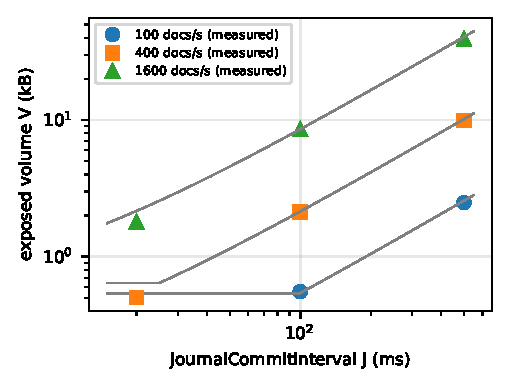
\includegraphics[width=\columnwidth]{figures/fig_plant.pdf}
\caption{Static plant: measured exposed volume versus $J$ at three loads, with the model (grey).}\label{fig:plant}
\end{figure}
\begin{table}[t]\centering\small
\caption{Static plant: measured exposed volume $V$ (kB per sync) versus the model $V=R(J+pL_0)/p$, $p=\min(1,RJ/b_0)$, $b_0=513$\,B, $L_0=7$\,ms.}\label{tab:plant}
\resizebox{\columnwidth}{!}{\begin{tabular}{rrrrrr}\toprule
Load (docs/s) & $J$ (ms) & $R$ (kB/s) & $V$ meas. & $V$ model & err. (\%)\\\midrule
100 & 500 & 5.1 & 2.49 & 2.57 & +3.4\\
100 & 100 & 5.1 & 0.56 & 0.54 & -2.3\\
100 & 20 & 5.0 & 0.50 & 0.54 & +6.9\\
400 & 500 & 20.0 & 9.92 & 10.16 & +2.4\\
400 & 100 & 20.0 & 2.13 & 2.14 & +0.7\\
400 & 20 & 20.0 & 0.50 & 0.64 & +27.8\\
1600 & 500 & 80.1 & 39.24 & 40.60 & +3.5\\
1600 & 100 & 80.0 & 8.58 & 8.57 & -0.1\\
1600 & 20 & 80.0 & 1.79 & 2.16 & +20.9\\
\bottomrule\end{tabular}}\end{table}


\paragraph{Dynamics.}
A load step from 400 to 1600 documents/s with $J$ fixed multiplied $V$ by 4.05 (at $J=100$\,ms) and 4.00
($J=200$\,ms) for a load ratio of 3.98. The 10\,s window makes the sensor the dominant dynamics: $V$ reaches 63\,\%
of its final value after 6.5--7\,s and 95\,\% after 10\,s, as expected for a moving average, whereas the
byte rate $R$ estimated tick by tick reaches 90\,\% after 2\,s. The actuator (\texttt{setParameter} plus read-back)
takes $4.9$\,ms on average (maximum 6.4\,ms), far below the 0.5\,s control period.

\paragraph{Measurement noise.}
The window average is noisy mainly because of counting: at $J=500$\,ms a 10\,s window contains about 20 syncs and one sync more or less changes $V$ by 5\,\%. The relative standard deviation of $V$
is \vcvMinFiveHundred--\vcvMaxFiveHundred\,\% at $J=500$\,ms, \vcvMinHundred--\vcvMaxHundred\,\% at 100\,ms and \vcvMinTwenty--\vcvMaxTwenty\,\% at 20\,ms (Table~\ref{tab:noise}). The per-tick
byte rate, used as load estimate, has a relative standard deviation of \rcvBaseMin--\rcvBaseMax\,\% at 400 documents/s and \rcvBurstMin--\rcvBurstMax\,\% at 1600, with a lag-one autocorrelation of
\racfBaseMin\ to \racfBaseMax\ (base) and \racfBurstMin\ to \racfBurstMax\ (burst): close to white, slightly negative because of tick-boundary counting. The noise is therefore a quantisation effect, not a drifting error,
and the steady-state error floor of 1.2--1.5\,\% seen in closed loop is of the same order.
\begin{table}[t]\centering\small
\caption{Measurement noise of the 10\,s signal $V$ (relative standard deviation over a 60\,s segment, open loop) and syncs per window.}\label{tab:noise}
\begin{tabular}{rrrr}\toprule
Load (docs/s) & $J$ (ms) & $\mathrm{sd}(V)/V$ (\%) & syncs per 10\,s\\\midrule
100 & 500 & 5.4 & 20\\
100 & 100 & 4.1 & 91\\
100 & 20 & 0.6 & 101\\
400 & 500 & 5.8 & 20\\
400 & 100 & 1.1 & 94\\
400 & 20 & 0.3 & 399\\
1600 & 500 & 5.8 & 20\\
1600 & 100 & 1.3 & 93\\
1600 & 20 & 0.4 & 448\\
\bottomrule\end{tabular}\end{table}


\section{Controllers and tuning}\label{sec:controllers}
All controllers work on $e=\ln V^*-\ln\hat V$ and command $J\in[20,500]$\,ms every 0.5\,s.
\paragraph{PI.} $u=u_0+K_p e+K_i\sigma$ with integrator $\sigma$, clamp or back-calculation anti-windup, and optional filtering of $\ln\hat V$.
\paragraph{Feedforward with observer (FF+obs).}
With $\hat R$ the smoothed per-tick byte rate, $J_\mathrm{ff}=V^*e^{-b}/\hat R-L_0$, where the bias
$b$ is an exponential average of $\ln V_{\rm measured}-\ln V_{\rm model}$ computed over the same 10\,s window; it
absorbs model error (floor, $p$, $L_0$) and compensates the sensor window. There is no feedback gain and no prediction.
\paragraph{PI with feedforward (PI-FF).} The same feedforward plus the PI correction; the tuner selected no bias observer for this family ($\text{bias}\_\alpha=0$) and unsmoothed load input.
\paragraph{MPC.} At each tick, $u=\ln J$ minimises $\sum_{i=1}^{H}\gamma^{i-1}s(e_i)e_i^2+\lambda(u-u_{\rm prev})^2$ with
$e_i=\ln V^*-[\ln v(\hat R_{k+i},e^{u})+b]$, $v$ the static law and $s=w$ when $V$ is below the target and 1 otherwise. $\hat R_{k+i}$ is
forecast by persistence (exponentially smoothed level), moving average (level plus least-squares slope) or ARIMA(1,1,0) fitted by least squares on the
window. The scalar problem is solved by grid search and golden-section refinement: with an additive linear model the cost is convex and a line search suffices, but with the static law $v$ convexity is not guaranteed, hence the continuous refinement of a dense grid. With a flat forecast, $H$ and $\lambda$ are redundant
($H e^2+\lambda\Delta^2 \equiv e^2+(\lambda/H)\Delta^2$) and MPC with $H=1$ reduces to FF+obs (checked numerically).

\paragraph{Tuning protocol.}
Each family (PI, PI-FF, FF+obs, and each MPC predictor) received the same budget of 60 random candidates, evaluated on a
calibrated simulator with a robust objective (half nominal plant, half stress plant with slower sync, more jitter and one tick of actuator delay),
on tuning seeds disjoint from test seeds. The three MPC predictors share the same candidates. Search ranges were widened after a first run placed continuous optima on an edge; the edge values that remain are the ``no filtering'' options (value 1) and extremes of discrete sets, listed with the tuned specifications in the repository. A first tuning gave the MPC an apparent advantage over PI-FF, traced to a different smoothing of the load estimate;
all controllers now receive the same raw inputs and tune their own smoothing. A PI with default gains is kept as a naive reference only. Table~\ref{tab:params} lists every parameter used.
\begin{table*}[t]\centering\small
\caption{Controller parameters used in all runs (random search, 60 candidates per family, robust objective; nominal values from the repository file \texttt{tuned\_specs.json}). PI-default is the naive reference (no tuning). Dashes: parameter not used by the family.}\label{tab:params}
\resizebox{\textwidth}{!}{\begin{tabular}{lccccccccccc}\toprule
Controller & $K_p$ & $K_i$ & anti-windup & $\alpha_V$ & feedforward & $\alpha_{R}$ & bias $\alpha_b$ & $H$ & $\gamma$ & $\lambda$ & $w$ (below target)\\\midrule
PI-default & 0.3 & 0.05 & clamp & 1 & no & -- & -- & -- & -- & -- & --\\
PI (tuned) & 3.19 & 0.35 & backcalc & 1 & no & -- & -- & -- & -- & -- & --\\
PI-FF & 3.66 & 0.19 & backcalc & 1 & yes & 1 & 0 & -- & -- & -- & --\\
FF+obs & 0.00 & 0.00 & clamp & 1 & yes & 1 & 1 & -- & -- & -- & --\\
MPC persistence & -- & -- & -- & -- & -- & 1 & 1 & 10 & 0.85 & 0.020 & 0.62\\
MPC moving average & -- & -- & -- & -- & -- & 0.3 & 1 & 3 & 0.7 & 0.024 & 0.86\\
MPC ARIMA(1,1,0) & -- & -- & -- & -- & -- & 0.3 & 1 & 3 & 0.7 & 0.024 & 0.86\\
\bottomrule\end{tabular}}
\\[2pt]{\footnotesize Common: $V^*=4096$\,B, period 0.5\,s, $J\in[20,500]$\,ms, $J_0=100$\,ms, window 10\,s, $b_0=513$\,B, $L_0=7$\,ms; MA/ARIMA window 5 / 5 samples (persistence ignores it). $\alpha_V$: filter on $\ln V$; $\alpha_R$: smoothing of the load estimate; $\alpha_b$: bias observer.}\end{table*}


\section{Experimental protocol}\label{sec:protocol}
\paragraph{Platform and workload.}
A Kind cluster (Kubernetes v1.27.3, one control plane and three workers) on a single Windows host under WSL2 (6\,GB), MongoDB 8.0.32 in a single
authenticated pod, other database workloads stopped. The generator inserts batches of 10 documents with four threads at a regulated rate,
write concern $w=1$, $j=\text{false}$. Target $V^*=4096$\,B.
\paragraph{Scenarios.} Stationary (400 documents/s); burst (400$\to$1600 documents/s from $t=100$ to 160\,s); low load (100$\to$400 documents/s, where $V^*$ is
unreachable at the start because $J$ would exceed 500\,ms). Runs last 300\,s with a 20\,s warm-up.
\paragraph{Design.} Controllers are run in randomised blocks (interleaved in time), 30\,s apart. A run is invalid and repeated if a pod restarts,
the acknowledged rate falls below 95\,\% of the offered rate, or insertions fail. A pilot of 63 runs (3 per cell) preceded a campaign of 71 runs; the pilot
used the same specifications and is pooled. Cell sizes were set after the pilot from its variability (amendment recorded before the campaign).
\paragraph{Pre-specified analysis.}
Primary criteria on the burst scenario: mean error during the burst and exposure peak (maximum over 2\,s windows, relative to $V^*$).
Seven contrasts, Mann--Whitney tests with Holm correction over 14 tests, Cliff's $\delta$ and bootstrap CIs; equivalence (TOST on Welch 90\,\% CI)
for the pairs where the claim is ``no difference'', with margins of 0.7 percentage points (burst error) and 0.10 (peak). Margins are about
half the steady-state noise floor.

\section{Results}\label{sec:results}
\paragraph{Data.}
135 main runs (pilot 63, campaign 71, one replacement run), all valid, plus 81 sensitivity runs, all valid; no pod restarted during any run, acknowledged/offered rate between 0.964 and 1.002. The pod was recreated once between the pilot and the campaign and restarted once between two sessions of the sensitivity campaign (13 runs before, 69 after; the concurrent nominal controls were run after).
\paragraph{Primary criteria.}
Table~\ref{tab:main} and Fig.~\ref{fig:burst}--\ref{fig:primary} summarise the burst scenario. The tuned PI has a burst error of \MaePITS\,\%\ (sd \MaeSdPITS) and a
peak of \PeakPITS$\times V^*$, against \MaePIFFS\,\% (PI-FF), \MaeFFOS\,\% (FF+obs) and \MaeMPCPS\,\% (MPC with persistence), with peaks of \PeakPIFFS, \PeakFFOS\ and
\PeakMPCPS. The PI-versus-PI-FF difference is $+$\cDMaePITPIFFS\ pp (95\,\% CI [\cLoMaePITPIFFS, \cHiMaePITPIFFS], $p_{\rm Holm}=\,$$\cPHMaePITPIFFS$).

\begin{figure}[t]\centering
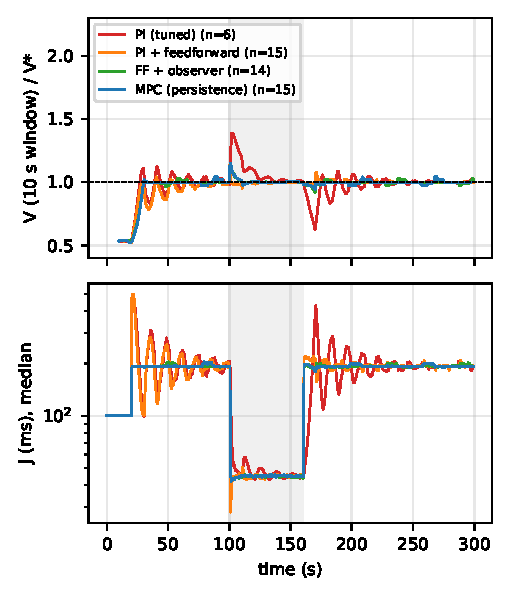
\includegraphics[width=\columnwidth]{figures/fig_burst.pdf}
\caption{Burst scenario, median over valid runs (shaded: burst). Top: $V$ over a 10\,s window relative to the target. Bottom: commanded $J$.}\label{fig:burst}
\end{figure}
\begin{figure*}[t]\centering
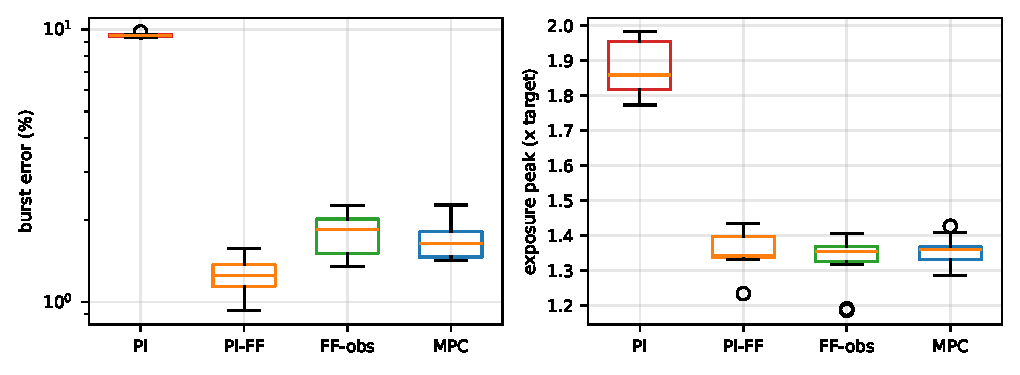
\includegraphics[width=0.8\textwidth]{figures/fig_primary.pdf}
\caption{Primary criteria per controller (boxes: quartiles; points: outliers).}\label{fig:primary}
\end{figure*}
\begin{table*}[t]\centering\small
\caption{Burst scenario (400$\to$1600 documents/s for 60 s): primary criteria and secondary measures, mean (sd) over $n$ valid runs (pilot included). The single run with a journal-sync stall $\geq 5$\,s (FF + observer) is excluded here; all contrasts are also reported with it (Table~\ref{tab:contrasts}). Peak = maximum exposure over 2\,s windows relative to the target $V^*$.}\label{tab:main}
\resizebox{0.92\textwidth}{!}{\begin{tabular}{lrcccc}\toprule
Controller & $n$ & Burst error (\%) & Peak ($\times V^*$) & Steady error (\%) & $|\Delta\ln J|$ per tick\\\midrule
PI (default gains) & 3 & 55.51 (1.80) & 2.71 (0.03) & 35.61 (0.65) & 0.005 (0.000)\\
PI (tuned) & 6 & 9.55 (0.15) & 1.88 (0.09) & 4.85 (0.13) & 0.043 (0.001)\\
PI + feedforward & 15 & 1.25 (0.17) & 1.36 (0.05) & 1.40 (0.10) & 0.055 (0.012)\\
FF + observer & 15 & 1.82 (0.30) & 1.34 (0.07) & 1.46 (0.11) & 0.032 (0.015)\\
MPC, persistence & 15 & 1.69 (0.28) & 1.36 (0.04) & 1.40 (0.12) & 0.026 (0.007)\\
MPC, moving average & 10 & 2.81 (0.45) & 1.50 (0.08) & 1.78 (0.25) & 0.024 (0.005)\\
MPC, ARIMA(1,1,0) & 10 & 1.83 (0.46) & 1.40 (0.14) & 1.59 (0.15) & 0.028 (0.009)\\
\bottomrule\end{tabular}}\end{table*}

\begin{table*}[t]\centering\small
\caption{Pre-specified contrasts (Mann--Whitney U, two-sided; Holm correction over the 14 tests = 7 contrasts $\times$ 2 primary criteria). Difference = mean(A) $-$ mean(B) with 95\% bootstrap CI; $\delta$ = Cliff's delta. ``All runs'' includes the stalled run; ``excl.'' removes it (post hoc sensitivity analysis).}\label{tab:contrasts}
\resizebox{\textwidth}{!}{\begin{tabular}{llccccc}\toprule
 & Contrast (A vs B) & Difference [95\% CI] (all runs) & $\delta$ & $p_{\text{Holm}}$ (all) & Difference [CI] (excl.) & $p_{\text{Holm}}$ (excl.)\\\midrule
\multicolumn{7}{l}{\emph{Burst error (pp)}}\\
 & PI vs PI-FF & +8.30 [+8.17, +8.44] & +1.00 & $4.4\!\times\!10^{-4}$ & +8.30 [+8.17, +8.44] & $4.4\!\times\!10^{-4}$\\
 & PI-FF vs FF+obs & -11.17 [-32.44, -0.44] & -0.93 & $1.8\!\times\!10^{-4}$ & -0.57 [-0.74, -0.40] & $2.7\!\times\!10^{-4}$\\
 & FF+obs vs MPC-pers. & +10.73 [-0.02, +32.03] & +0.35 & $0.605$ & +0.13 [-0.07, +0.32] & $0.951$\\
 & PI-FF vs MPC-pers. & -0.44 [-0.61, -0.29] & -0.92 & $2.5\!\times\!10^{-4}$ & -0.44 [-0.61, -0.29] & $2.7\!\times\!10^{-4}$\\
 & MPC-pers. vs MPC-MA & -1.12 [-1.42, -0.83] & -0.95 & $9.2\!\times\!10^{-4}$ & -1.12 [-1.42, -0.83] & $9.2\!\times\!10^{-4}$\\
 & MPC-pers. vs MPC-ARIMA & -0.14 [-0.43, +0.17] & -0.15 & $1.000$ & -0.14 [-0.43, +0.17] & $1.000$\\
 & PI vs MPC-pers. & +7.86 [+7.68, +8.03] & +1.00 & $4.4\!\times\!10^{-4}$ & +7.86 [+7.68, +8.03] & $4.4\!\times\!10^{-4}$\\
\multicolumn{7}{l}{\emph{Peak ($\times V^*$)}}\\
 & PI vs PI-FF & +0.52 [+0.45, +0.59] & +1.00 & $0.005$ & +0.52 [+0.45, +0.59] & $0.005$\\
 & PI-FF vs FF+obs & -2.33 [-7.07, +0.05] & +0.10 & $1.000$ & +0.02 [-0.01, +0.06] & $1.000$\\
 & FF+obs vs MPC-pers. & +2.34 [-0.05, +7.07] & +0.06 & $1.000$ & -0.02 [-0.06, +0.01] & $1.000$\\
 & PI-FF vs MPC-pers. & +0.00 [-0.03, +0.03] & +0.09 & $1.000$ & +0.00 [-0.03, +0.03] & $1.000$\\
 & MPC-pers. vs MPC-MA & -0.15 [-0.20, -0.09] & -0.81 & $0.005$ & -0.15 [-0.20, -0.09] & $0.005$\\
 & MPC-pers. vs MPC-ARIMA & -0.04 [-0.13, +0.04] & -0.25 & $1.000$ & -0.04 [-0.13, +0.04] & $1.000$\\
 & PI vs MPC-pers. & +0.52 [+0.46, +0.59] & +1.00 & $0.005$ & +0.52 [+0.46, +0.59] & $0.005$\\
\bottomrule\end{tabular}}\end{table*}


\paragraph{MPC versus feedforward with observer.}
FF+obs versus MPC with persistence: $+$\cDMaeFFOMPCPS\ pp [\cLoMaeFFOMPCPS, \cHiMaeFFOMPCPS] on the burst error ($p_{\rm Holm}=\,$$\cPHMaeFFOMPCPS$) and
\cDPeakFFOMPCPS\ on the peak. The equivalence tests (Table~\ref{tab:equiv}) conclude to equivalence on both criteria once the stalled run (below) is set aside, and are
inconclusive with it (one extreme value widens the CI), while the rank tests do not change.
MPC with a moving average has a burst error larger than persistence by \cAMaeMPCPMPCMS\ pp, and ARIMA is equivalent to persistence on the burst error;
neither forecaster improves on persistence.
\begin{table}[t]\centering\small
\caption{Equivalence tests (TOST, Welch 90\% CI inside $\pm$ margin; margins 0.7\,pp on the burst error and 0.10 on the peak).}\label{tab:equiv}
\resizebox{\columnwidth}{!}{\begin{tabular}{lccc}\toprule
Pair, criterion & 90\% CI (excl.) & verdict (excl.) & verdict (all)\\\midrule
FF+obs vs MPC-pers., error & [-0.05, +0.31] & equivalent & inconclusive\\
MPC-pers. vs MPC-ARIMA, error & [-0.42, +0.15] & equivalent & equivalent\\
FF+obs vs MPC-pers., peak & [-0.05, +0.01] & equivalent & inconclusive\\
MPC-pers. vs MPC-ARIMA, peak & [-0.12, +0.04] & inconclusive & inconclusive\\
\bottomrule\end{tabular}}\end{table}


\paragraph{PI with feedforward.}
PI-FF has the lowest burst error, \cAMaePIFFMPCPS\ pp below MPC (Table~\ref{tab:contrasts}), with no difference on the exposure peak. It also moves $J$ about twice as much
(\ChatPIFFS\ against \ChatMPCPS\ in $|\Delta\ln J|$ per tick) and, when the target is unreachable and the actuator saturates (low-load scenario), recovers in \LowRecPIFFS\,s against \LowRecMPCPS\,s
for MPC (Table~\ref{tab:other}).
\begin{table}[t]\centering\small
\caption{Stationary (400 documents/s) and low-load (100$\to$400 documents/s, target unreachable at the start) scenarios, mean over $n$ runs.}\label{tab:other}
\resizebox{\columnwidth}{!}{\begin{tabular}{lcccc}\toprule
Controller & Stat. err. (\%) & Low-load err. (\%) & Recov. (s) & $n$\\\midrule
PI-def. & 26.08 & 49.83 & -- & 3\\
PI & 1.32 & 28.78 & 1.8 & 6\\
PI-FF & 1.38 & 31.48 & 24.1 & 6\\
FF+obs & 1.34 & 28.18 & 2.9 & 6\\
MPC-pers. & 1.22 & 28.01 & 3.0 & 6\\
MPC-MA & 1.31 & 28.22 & 2.3 & 6\\
MPC-ARIMA & 1.49 & 28.27 & 2.8 & 6\\
\bottomrule\end{tabular}}\end{table}


\paragraph{A journal-sync stall.}
One run (FF+obs, first run after the pod was recreated) shows no journal sync for 12.5\,s during the burst, then 1.5\,s and 1\,s; its burst error is 171\,\% and its peak $39\times V^*$. It is valid under the
pre-specified rules and is included in the primary analysis; the sensitivity analysis excludes runs with a sync gap of 5\,s or more (a rule defined from the counters, post hoc). The cause is unknown; four
shorter gaps (1--1.5\,s) occur in two other runs. Counters of journal pre-allocation are now recorded to investigate such events.

\paragraph{Simulator versus real cluster.}
The simulator was calibrated on the static grid (worst error 3.9\,\% on $V$) and on the burst response. On the pilot the ranking of the seven controllers by burst error is identical to the simulated
one (Spearman 1.00), with real-to-simulated ratios between 0.80 and 1.09. The simulator underestimates the steady-state measurement noise (real error 1.2--1.5\,\% versus 0.5--0.95\,\%) and the between-run variability,
so it was used for tuning and design only.

\subsection{Sensitivity to parameters and to the target}
The criteria below were fixed before the runs (amendment 2). Each continuous parameter of PI, PI-FF, FF+obs and MPC (persistence) was perturbed one at a time by $\times0.5$ and $\times1.5$ (clipped to valid values), 3 runs per variant, with 3 concurrent nominal runs per controller
(Table~\ref{tab:sens}); the target was also changed (Table~\ref{tab:vstar}). The analysis is descriptive ($n=3$): ranges and ratios, no tests.
\paragraph{C1, parameter robustness.}
Worst ratio of burst error to the concurrent nominal: PI \SensWorstPIT, FF+obs \SensWorstFFO, MPC \SensWorstMPCP, PI-FF \SensWorstPIFF. For FF+obs, MPC and PI-FF the large ratios come from one parameter, the smoothing of the load estimate:
halving its factor multiplies the burst error by \SensSmoothFFO\ (FF+obs), \SensSmoothMPCP\ (MPC) and \SensSmoothPIFF\ (PI-FF). The MPC weights ($\lambda$, $w$) and the observer factor change the error by $-10$ to $+16$\,\%.
PI-FF is the only controller that loses stability: with $K_p\times1.5$ ($K_p=5.5$) it oscillates, with a burst error of \SensPIFFkpErr\,\% and a peak of \SensPIFFkpPeak$\times V^*$.
\paragraph{C2, robustness of the ranking.}
On the burst error the worst load-aware variant (\SensWorstAwareErr\,\%) is below the best PI variant (\SensBestPIErr\,\%): the ranking survives. On the exposure peak it survives for FF+obs (largest peak \SensMaxPeakFFO) and for MPC (\SensMaxPeakMPCP)
against the best PI variant (\SensMinPeakPIT) but not for PI-FF (\SensPIFFkpPeak). As specified, over the union of the three load-aware families, C2 is therefore \emph{not} satisfied on the peak; we report it as such.
\paragraph{C3, target.}
Journal syncs per second follow $1/V^*$ (about 17, 8.6 and 4.3 per second for $V^*=2048$, 4096 and 8192\,B, Table~\ref{tab:vstar}), the cost of a tighter target. No controller is uniformly best across targets;
at the unreachable $V^*=2048$\,B the MPC has a larger error than FF+obs.
\begin{table}[t]\centering\small
\caption{Sensitivity to controller parameters (burst scenario, $n=3$ per variant, one-at-a-time, descriptive). Ratios are relative to 3 concurrent nominal runs of the same controller. Nominal: PI \MaeSensPITnom\,\%, PI-FF \MaeSensPIFFnom\,\%, FF+obs \MaeSensFFOnom\,\%, MPC \MaeSensMPCPnom\,\%.}\label{tab:sens}
\resizebox{\columnwidth}{!}{\begin{tabular}{llcccc}\toprule
Controller & Variant & Error (\%) & Ratio & Peak ($\times V^*$) & $|\Delta\ln J|$\\\midrule
PI & $K_i\times0.5$ & 14.79 & 1.58 & 1.82 & 0.041\\
PI & $K_i\times1.5$ & 8.07 & 0.86 & 2.08 & 0.048\\
PI & $K_p\times0.5$ & 11.35 & 1.21 & 2.16 & 0.024\\
PI & $K_p\times1.5$ & 8.52 & 0.91 & 1.77 & 0.063\\
PI-FF & $\alpha_R\times0.5$ & 2.44 & 2.16 & 1.47 & 0.048\\
PI-FF & $K_i\times0.5$ & 2.98 & 2.63 & 1.32 & 0.057\\
PI-FF & $K_i\times1.5$ & 1.33 & 1.18 & 1.42 & 0.059\\
PI-FF & $K_p\times0.5$ & 1.47 & 1.30 & 1.33 & 0.043\\
PI-FF & $K_p\times1.5$ & 4.76 & 4.20 & 7.45 & 0.094\\
FF+obs & $\alpha_b\times0.5$ & 1.68 & 1.02 & 1.41 & 0.029\\
FF+obs & $\alpha_R\times0.5$ & 3.18 & 1.93 & 1.54 & 0.016\\
MPC-pers. & $\alpha_b\times0.5$ & 1.43 & 0.90 & 1.36 & 0.020\\
MPC-pers. & $\alpha_R\times0.5$ & 3.70 & 2.32 & 1.61 & 0.023\\
MPC-pers. & $\lambda\times0.5$ & 1.85 & 1.16 & 1.37 & 0.032\\
MPC-pers. & $\lambda\times1.5$ & 1.49 & 0.93 & 1.33 & 0.023\\
MPC-pers. & $w\times0.5$ & 1.51 & 0.95 & 1.33 & 0.026\\
MPC-pers. & $w\times1.5$ & 1.47 & 0.92 & 1.42 & 0.023\\
\bottomrule\end{tabular}}\end{table}

\begin{table}[t]\centering\small
\caption{Change of the target $V^*$ (burst, $n=3$): error, peak and journal syncs per second. At $V^*=2048$\,B the target is unreachable during the burst ($J$ would be below 20\,ms).}\label{tab:vstar}
\begin{tabular}{llccc}\toprule
Controller & $V^*$ (B) & Error (\%) & Peak & syncs/s\\\midrule
PI-FF & 2048 & 2.33 & 1.34 & 17.02\\
PI-FF & 4096 & 1.13 & 1.40 & 8.68\\
PI-FF & 8192 & 2.32 & 1.47 & 4.41\\
FF+obs & 2048 & 1.74 & 1.32 & 17.23\\
FF+obs & 4096 & 1.64 & 1.39 & 8.62\\
FF+obs & 8192 & 2.83 & 1.40 & 4.31\\
MPC-pers. & 2048 & 4.90 & 1.57 & 16.76\\
MPC-pers. & 4096 & 1.60 & 1.37 & 8.61\\
MPC-pers. & 8192 & 3.68 & 1.39 & 4.28\\
\bottomrule\end{tabular}\end{table}


\section{Discussion}\label{sec:discussion}
\paragraph{Why prediction does not help here.}
The actuator acts on $V$ within one control tick, while the sensor is delayed by the 10\,s window. A controller that knows $\hat R$ and the static law can therefore set $J$ almost
exactly; what remains is to correct the sensor lag and model error, which the bias observer does. Forecasting $R$ several ticks ahead adds noise, not information, because the plant has no
delay to compensate: with a moving average the burst error is worse. This is consistent with the equivalence of MPC and FF+obs.
\paragraph{Why feedback alone fails.}
Feedback on the windowed $V$ reacts only as the window fills. Even with a high proportional gain ($K_p=3.2$, $K_i=0.35$ after tuning) the PI shows a
burst error five to eight times larger than PI-FF, FF+obs and MPC with persistence, and a peak 1.4 times higher (Fig.~\ref{fig:burst}); its response oscillates around the target.
\paragraph{What matters.}
The controller structure matters less than the responsiveness of the load estimate: smoothing it more than the plant requires doubles the burst error for every load-aware controller (Table~\ref{tab:sens}), while the MPC weights and the observer factor are second order.
\paragraph{Practical guidance.}
On this engine and knob, a load feedforward with a model-bias observer is the simplest controller that attains the accuracy of MPC and it was stable over every perturbation tested. PI with feedforward has the lowest nominal burst error but the least margin: a 50\,\% higher gain made it oscillate,
and it moves the actuator twice as much and recovers more slowly under saturation. We therefore see feedback as optional: useful only with a gain margin that is measured, not assumed.

\section{Limitations}\label{sec:limits}
(i) One engine, one single-pod deployment and one Kind host under WSL2; (ii) $V$ is a composite of two counters and no crash-recovery experiment verifies it as data loss;
(iii) the simulator underestimates noise and between-run variability; (iv) tuning was done on the simulator and checked on a pilot; (v) one run contains a long journal-sync stall of unknown cause;
(vi) the simulator reproduces the nominal behaviour but not the fragility of PI-FF near its stability limit (a 50\,\% higher gain does not oscillate in simulation unless one extra tick of delay is added, which reproduces it qualitatively), so unmodelled delay is a plausible but unverified cause; (vii) the pod restarted once between two sessions of the sensitivity campaign (each run individually valid); (viii) equivalence margins are set from the noise floor and a different margin could change an ``inconclusive'' into ``equivalent'' or the reverse; (ix) the sensitivity analysis is descriptive ($n=3$ per variant) and one-at-a-time, so interactions between parameters are not explored.

\section{Conclusion}\label{sec:conclusion}
On a real MongoDB cluster, using the observed write load is what lets a controller hold the exposed journal volume near its target during bursts. A model predictive controller with persistence forecasting is equivalent to a plain
feedforward with a model-bias observer, and forecasting the load with a moving average or ARIMA does not help. The advantage of the feedforward does not depend on a precise tuning, except for the responsiveness of the load estimate, and a feedback term must be added with a measured gain margin. These conclusions are limited to the scenarios, engine and platform tested.

\begin{acknowledgements}
\todo{acknowledgements, if any}
\end{acknowledgements}

\section*{Declarations}
\textbf{Funding.} No funding was received. \textbf{Competing interests.} The authors declare no competing interests.
\textbf{Data and code availability.} \todo{insert the public repository URL after publishing the code (mpcrpo), the 134+ run files, the schedules and the analysis scripts; the earlier repository does not contain them}.
\textbf{Use of AI tools.} \todo{describe, as required by the target journal, any use of AI assistance in code, analysis or writing}.

\begin{thebibliography}{9}
\bibitem{camacho2013model}
E.\ F.\ Camacho and C.\ Bordons.
\newblock \emph{Model Predictive Control}.
\newblock Advanced Textbooks in Control and Signal Processing.
  Springer-Verlag London, 2nd edition, 2007.

\bibitem{muske2002disturbance}
K.\ R.\ Muske and T.\ A.\ Badgwell.
\newblock Disturbance modeling for offset-free linear model predictive
  control.
\newblock \emph{Journal of Process Control}, 12(5):617--632, 2002.

\bibitem{pannocchia2003disturbance}
G.\ Pannocchia and J.\ B.\ Rawlings.
\newblock Disturbance models for offset-free model-predictive control.
\newblock \emph{AIChE Journal}, 49(2):426--437, 2003.

\bibitem{kothare1994antiwindup}
M.\ V.\ Kothare, P.\ J.\ Campo, M.\ Morari, and C.\ N.\ Nett.
\newblock A unified framework for the study of anti-windup designs.
\newblock \emph{Automatica}, 30(12):1869--1883, 1994.

\bibitem{astrom1989windup}
K.\ J.\ {\AA}str\"om and L.\ Rundqwist.
\newblock Integrator windup and how to avoid it.
\newblock In \emph{Proceedings of the 1989 American Control
  Conference}, pp.\ 1693--1698. IEEE, 1989.

\bibitem{roy2011autoscaling}
N.\ Roy, A.\ Dubey, and A.\ Gokhale.
\newblock Efficient autoscaling in the cloud using predictive models
  for workload forecasting.
\newblock In \emph{Proceedings of the IEEE 4th International
  Conference on Cloud Computing (CLOUD'11)}, pp.\ 500--507, 2011.

\bibitem{gong2010press}
Z.\ Gong, X.\ Gu, and J.\ Wilkes.
\newblock PRESS: PRedictive Elastic ReSource Scaling for cloud
  systems.
\newblock In \emph{Proceedings of the International Conference on
  Network and Service Management (CNSM)}, pp.\ 9--16, 2010.

\bibitem{cai2022inverse}
Z.\ Cai and R.\ Buyya.
\newblock Inverse queuing model-based feedback control for elastic
  container provisioning of web systems in Kubernetes.
\newblock \emph{IEEE Transactions on Computers}, 71(2):337--348, 2022.

\bibitem{pozdniakova2024sla}
O.\ Pozdniakova, D.\ Ma\v{z}eika, and A.\ Cholomskis.
\newblock SLA-adaptive threshold adjustment for a Kubernetes
  horizontal pod autoscaler.
\newblock \emph{Electronics}, 13(7):1242, 2024.

\bibitem{serracanta2025stability}
B.\ Serracanta, A.\ Luk\'acs, A.\ Rodriguez-Natal, A.\ Cabellos, and
  G.\ R\'etv\'ari.
\newblock On the stability of the Kubernetes horizontal autoscaler
  control loop.
\newblock \emph{IEEE Access}, 13:7160--7166, 2025.

\bibitem{baresi2016discrete}
L.\ Baresi, S.\ Guinea, A.\ Leva, and G.\ Quattrocchi.
\newblock A discrete-time feedback controller for containerized cloud
  applications.
\newblock In \emph{Proceedings of the 24th ACM SIGSOFT International
  Symposium on Foundations of Software Engineering (FSE 2016)}, pp.\
  217--228, 2016.

\bibitem{sabuhi2021adaptive}
M.\ Sabuhi, N.\ Mahmoudi, and H.\ Khazaei.
\newblock Optimizing the performance of containerized cloud software
  systems using adaptive PID controllers.
\newblock \emph{ACM Transactions on Autonomous and Adaptive Systems},
  15(3), 2021.

\bibitem{vanaken2017ottertune}
D.\ Van Aken, A.\ Pavlo, G.\ J.\ Gordon, and B.\ Zhang.
\newblock Automatic database management system tuning through
  large-scale machine learning.
\newblock In \emph{Proceedings of the 2017 ACM International
  Conference on Management of Data (SIGMOD'17)}, pp.\ 1009--1024, 2017.

\bibitem{zhang2019cdbtune}
J.\ Zhang, Y.\ Liu, K.\ Zhou, G.\ Li, Z.\ Xiao, B.\ Cheng, J.\ Xing,
  Y.\ Wang, T.\ Cheng, L.\ Liu, M.\ Ran, and Z.\ Li.
\newblock An end-to-end automatic cloud database tuning system using
  deep reinforcement learning.
\newblock In \emph{Proceedings of the 2019 ACM International
  Conference on Management of Data (SIGMOD'19)}, pp.\ 415--432, 2019.

\bibitem{ferreira2020selftunable}
L.\ Ferreira, F.\ Coelho, and J.\ Pereira.
\newblock Self-tunable DBMS replication with reinforcement learning.
\newblock In \emph{Distributed Applications and Interoperable Systems
  (DAIS 2020)}, LNCS vol.\ 12135, pp.\ 131--147. Springer, 2020.

\bibitem{joshi2024arimapid}
N.\ S.\ Joshi, R.\ Raghuwanshi, Y.\ M.\ Agarwal, B.\ Annappa, and
  D.\ N.\ Sachin.
\newblock ARIMA-PID: container auto scaling based on predictive
  analysis and control theory.
\newblock \emph{Multimedia Tools and Applications}, 83(9):26369--26386,
  2024.

\bibitem{kusic2009lookahead}
D.\ Kusic, J.\ O.\ Kephart, J.\ E.\ Hanson, N.\ Kandasamy, and G.\ Jiang.
\newblock Power and performance management of virtualized computing
  environments via lookahead control.
\newblock \emph{Cluster Computing}, 12(1):1--15, 2009.

\bibitem{padala2009automated}
P.\ Padala, K.-Y.\ Hou, K.\ G.\ Shin, X.\ Zhu, M.\ Uysal, Z.\ Wang,
  S.\ Singhal, and A.\ Merchant.
\newblock Automated control of multiple virtualized resources.
\newblock In \emph{Proceedings of the 4th ACM European Conference on
  Computer Systems (EuroSys'09)}, pp.\ 13--26, 2009.

\bibitem{fang2016qos}
Q.\ Fang, J.\ Wang, and Q.\ Gong.
\newblock QoS-driven power management of data centers via model
  predictive control.
\newblock \emph{IEEE Transactions on Automation Science and
  Engineering}, 13(4):1557--1566, 2016.
\end{thebibliography}
\end{document}
